% This file was made by Davide M.
% I imagine a lot of you will read this file to use as an example:
% beware, not all the features present in LaTeX have been used here.
% First of all, this is an input file, it won't compile on its own, this is
% how all the chapters will look like once the formulary is done, for now
% if you are still developing your chapter, keep using the \begin{document}...\end{document}
% environment, it will make it such that you'll be able to compile your file on its own.
% If you want to see how to produce a "proper" (ngl that is a bit of a mess) preamble,
% go look at the start of notes.tex

% So, fundamentally to give a command you use the "\" sign: it will be your best friend.
% Almost anything which is not in contact with that sign (or to characters
% in contact to that sign) will be regarded as actual text.
% To give arguments to commands: {} are used, those arguments are usually text itself, like in
% \emph{Hello!} (emph stands for "emphasize", it makes the text italic), but can
% sometimes be actual values. (In some particular cases, see as example \sqrt[]{}, even []
% can be used to pass arguments)
% To enter math-mode there are two ways:
%   -Inline math is done $...$, it will try to write math-text by following the paragraph lines.
%   -Outline (don't know the name) math is done in multiple ways, mainly through the "equation"
%       environment.

% Finally, as you'll see in the file, text is divided into Sections, Subsections, Paragraphs and Subparagraphs.
% Sections and Subsections will be seen inside the Index at the beginning of the notes.tex
% final file, so be sure to insert important and meaningful names in there.
% Paragraphs and subparagraphs are less defined, but try to keep sense of what you are doing.

\section{Vectors}
\epigraph{Geometric entity characterized by a magnitude and a direction.}{A vector's minimal definition, Wikipedia}
% Don't mind this heart's-inspiring quote- but if you want to make one, use \epigraph
\begin{wrapfigure}{l}{0.25\textwidth}
    \input{chapters/vectors/images/vector_basic.pdf_tex}
    % As you can see here the input is given by following the folders starting from the main
    % folder, where notes.tex is: this is because, since this piece of text is actually run
    % itself from an \input in the notes.tex, this code has to be aware of that.
    %
    % Also don't be afraid of the fact I added figures in this text, this is mainly to give you
    % an example, there is no problem if no images in your chapter! (If you want to add some
    % though, be prepared to use the graphix package, if you also want to make them ad-hoc be 
    % prepared to use Inkscape, I use that at least.)
\end{wrapfigure}
\paragraph{What is a vector} In its fundamental concept, a vector is the transformation needed to move from one point (usually the origin) in space to another, in physics, it is mainly used to describe quantities that are bound to multiple dimensions, like movement or force. Dimensionless quantities, like temperature or mass, are instead defined through natural numbers, more correctly called \emph{scalars}.
\subsection{How to represent vectors} There are two main ways to represent vectors, the Magnitude-Angle notation and the Component notation: through experience, one may learn when to prefer the use of one over the other.
\paragraph{Magnitude-Angle} It describes (in a two-dimensional space) the vector as a pair $\langle m, \sigma\rangle$, where $|v|=m$ is the magnitude (or length) of the vector bound as $0\le m \le +\infty$ (a length can't be negative) and $\sigma$ is its direction (or angle) bound as $0=\SI{0}{\degree}\le \sigma \le 2\pi = \SI{360}{\degree}$.
\begin{equation}
    \vec{v} =\begin{cases}
        % The cases environment is used to write multiline curly brackets:
        % like in a multichoice function or a system of equations.
        m \mbox{ - Magnitude}\\ % This is the first forced newline!, as you can see you do that
        \sigma \mbox{ - Angle}  % by writing \\. Also you can write text in math-mode by doing
    \end{cases}                 % \mbox (if you want to write function names use \mathrm{})
\end{equation}
\paragraph{Component notation} Represents the vector as a linear sum of scalar products between the coordinates' unit vectors.
\begin{equation}
    \vec{v} = v_x \hat{i} + v_y \hat{j}\equiv \begin{bmatrix}   
        v_x\\ v_y
    \end{bmatrix} % The bmatrix environment can be used to print vectors and matrices.
\end{equation}
In this case the scalars are unbounded across $\mathbb{R}$, they can hold any value.
\paragraph{Changing notation} Being possible to represent a vector in both ways, it is possible to switch from one notation to the other.
\begin{equation}
    \begin{cases}
        m = \sqrt{v_x^2 +v_y^2}\\
        \sigma = \tan\frac{v_y}{v_x}
    \end{cases}
    \iff
    \begin{cases}
        v_x = m \cos \sigma\\
        v_y = m \sin \sigma
    \end{cases}
\end{equation}
\paragraph{Unit vectors} A unit vector is any vector with magnitude $|v|=1$. In Magnitude-Angle notation, just let the magnitude equal to $1$. In Component notation, divide through scalar multiplication on its magnitude.
\begin{equation}
    \hat{v} = \begin{cases}
        |v| = 1 \mbox{ - Magnitude-Angle notation}\\
        \frac{1}{|v|} \vec{v} \mbox{ - Component notation}
    \end{cases}
\end{equation}
\subparagraph{Coordinates of a space} To represent vectors in any space with $n$-dimensions at least $n$ coordinate vectors are needed: the most commonly used set of these is $\langle \hat{i}, \hat{j}, \hat{k}\rangle$ (for three dimensions, just $\hat{i}, \hat{j}$ for two), which are unit vectors holding properties between each other (orthogonality, etc.) such that they can form a basis (can be used to represent any vector) for the space they are in.
\begin{equation}
    \hat{i} =\begin{bmatrix}1\\0\\0\end{bmatrix} \quad
    \hat{j} =\begin{bmatrix}0\\1\\0\end{bmatrix} \quad
    \hat{k} =\begin{bmatrix}0\\0\\1\end{bmatrix}
\end{equation}
\subsection{Operations on vectors} As we've just seen, vectors may be represented in multiple ways: this is why, when describing operations, we'll sometimes define two processes.
\paragraph{Vector negation} The only unary operation, returns a vector holding same magnitude but opposite direction:
\begin{equation}
    -\vec{v} = \begin{cases}
        \langle m, \sigma + \pi\rangle \mbox{ -Mag/Angl}\\
        (-v_x, -v_y) \mbox{ -Comp.}
    \end{cases}
\end{equation}
\paragraph{Vector sum $+$} We've previously said how a vector represents the movement from one point to another: the result of summing vectors is a vector representing movement from a starting point to an ending point if multiple movements happened.
\begin{equation}
    \vec{a} + \vec{b} = (a_x + b_x, a_y + b_y)
\end{equation}
This is one of the few cases in which to compute the operation just one representation is usable, the Component one: indeed to compute through Magnitude-Angle representation we first need to switch into Component notation and back again with the result.\\
This operation holds both the commutativity and the associativity law.
\paragraph{Scalar multiplication} Binary operation taking a scalar value and a vector: the result has its magnitude equal to the product of the original vector's magnitude and the scalar value. Since a magnitude can't be negative if the scalar value is negative the direction of the resulting vector will be opposite to the original one.
\begin{equation}
    a\vec{v} = \begin{cases}
        \langle|am|, \texttt{if } a\ge0:\sigma\texttt{ otherwise }\sigma+\pi\rangle\mbox{ -Mag/Angl}\\
        (av_x, av_y)\mbox{ -Comp.}
    \end{cases}
\end{equation}
\paragraph{Dot product $\cdot$} Instinctively speaking, the dot product is an operation which returns a scalar representing the similarity of two vectors: indeed, if two vectors are parallel, their dot product will be equal to the product of their magnitudes, while if they are orthogonal (perpendicular) the result will default to $0$.
\begin{equation}
    \vec{a}\cdot\vec{b} = \begin{cases}
        |a||b|\cos(\phi)\mbox{ -Mag/Angl}\\
        a_xb_x+a_yb_y\mbox{ -Comp.}
    \end{cases}
\end{equation}
The angle between the two vectors $\phi$ can be found by computing:
\begin{equation}
    \cos(\phi) = \frac{\vec{a}\cdot\vec{b}}{|a||b|}
\end{equation}
As we can see, if that angle is not given then the dot product is better found by using Component notation.\\
The dot product too holds the commutativity and distributivity law, furthermore, if any scalar value is multiplying one of the two vectors, that can be taken out of the operation and multiplied to the result.
\begin{equation}
    \vec{a}\cdot(k\vec{b}) = k(\vec{a}\cdot\vec{b})
\end{equation}
\paragraph{Cross product $\times$} Maybe the most important operation on vectors, returns a vector orthogonal to the input vectors and with magnitude proportional to the orthogonality of the two inputs: that is, if the two vectors are parallel it is $0$, while it will be equal to the product of the two input magnitudes if they are perpendicular.
\begin{equation}
    \vec{a}\times\vec{b} = \begin{cases}
        \langle |a||b|\sin(\phi), \sigma\mbox{ ortho. to inputs}\rangle\mbox{ -Mag/Angl}\\
        \begin{vmatrix}
            \hat{i}&\hat{j}&\hat{k}\\
            a_x&a_y&a_z\\
            b_x&b_y&b_z
        \end{vmatrix}= (a_yb_z-a_zb_y)\hat{i} - (a_xb_z-a_zb_x)\hat{j} + (a_xb_y-a_yb_x)\hat{k}
    \end{cases}
\end{equation}
The distributivity law holds for the cross product, but does \textbf{not} with the commutativity law: we can see it through the so-called \emph{right-hand rule}. Furthermore, here too constants multiplied to our vectors can be brought outside the operation.

\begin{wrapfigure}{r}{0.3\textwidth}
    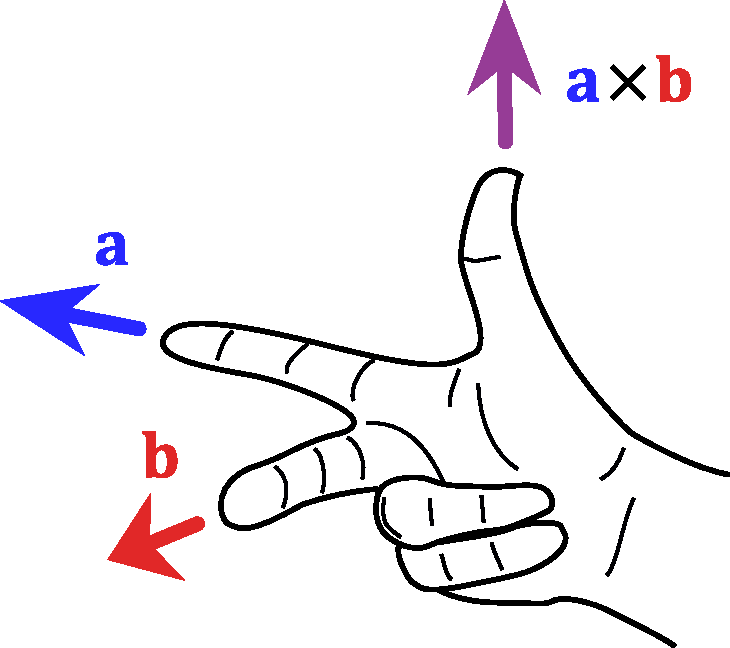
\includegraphics[width=0.3\textwidth]{chapters/vectors/images/right_hand_rule.pdf}
\end{wrapfigure}
\subparagraph{Right-hand rule} The right-hand rule is a simple way to imagine the direction of the vector resulting off a cross product, indeed it is not easy to find it through the Magnitude-Angle notation, nor it is so through Component notation (even though by crunching the numbers it is possible to do so). If done well it is possible to visualize how impossible it is to process the same result by switching the arguments: spoiler it would be of the opposite direction.